%!TEX root = ../dissertation.tex

\chapter{Implementing Programming Tools for Generative Design}
\label{chapter:evaluation}

This chapter presents a coherent implementation of the proposed programming tools exploring the ideas suggested in the previous sections. The first part describes the design decisions which affected the course of development, focusing on the rationale behind them. The second part shows the achieved result, detailing technical aspects of the software architecture. The last part describes the performed test conducted with target users, to test the initial hypothesis.

\section{Rosetta}

Due to time constraints, among other factors, an early decision was to opt for extending an existing programming environment, rather than implement one from scratch. This decision is critical due to its consequences especially on the implementation effort. Moreover, a \gls{gd} system that does not respect the main design principles discussed in this thesis can ruin the purpose of any tool build on top of it. Thus, to choose an adequate system to extend,
a comparative study was devised evaluating the potential choices in three design principles, which I consider successful designs for a \gls{gd} system. These principles are (1) portability of programs, (2) language independence, and (3) a strong correlation between programs and models. From the set systems that I analyzed, Rosetta~\citep{lopes2011portable} was the system that more strictly implements these principles. Therefore, I chose Rosetta as a basis for implementing the interactive programming tools proposed previously.

Rosetta is undoubtedly a distinct programming system, and it provides a modern environment for \gls{gd}, designed to overcome the limitations of the most used \gls{gd} systems. One of the most important limitations concerns is the portability of programs that are written in programming languages provided by \gls{gd} systems. For example, a RhinoScript program will execute in different versions of Rhinoceros3D \glspl{cad}. However, it will not run in AutoCAD. In this case, users must translate their programs to a programming language that is supported by the target \gls{gd} system. Translating programs might be a common task for a software engineer, but it is an ambitious and error-prone task for a designer. Unable to overcome this limitation, designers become locked-in to a particular family of \gls{cad} applications and cannot reuse programs of different families.

Rosetta overcomes this problem by providing (1) multiple programming languages as \textit{frontends}, from where users can choose to write their \gls{gd} programs; and (2) multiple \gls{cad} applications as \textit{backends}, which are used to
display the geometric models. For example, Figure~\ref{fig:rosetta-gui} shows Rosetta with a Racket program and its corresponding geometry in AutoCAD. Using Rosetta the geometric model becomes portable, which means that it has no dependency of any \gls{cad} application, neither any \gls{cad} particular programming language, becoming highly customizable.

\begin{figure}[!h]
  \centering
  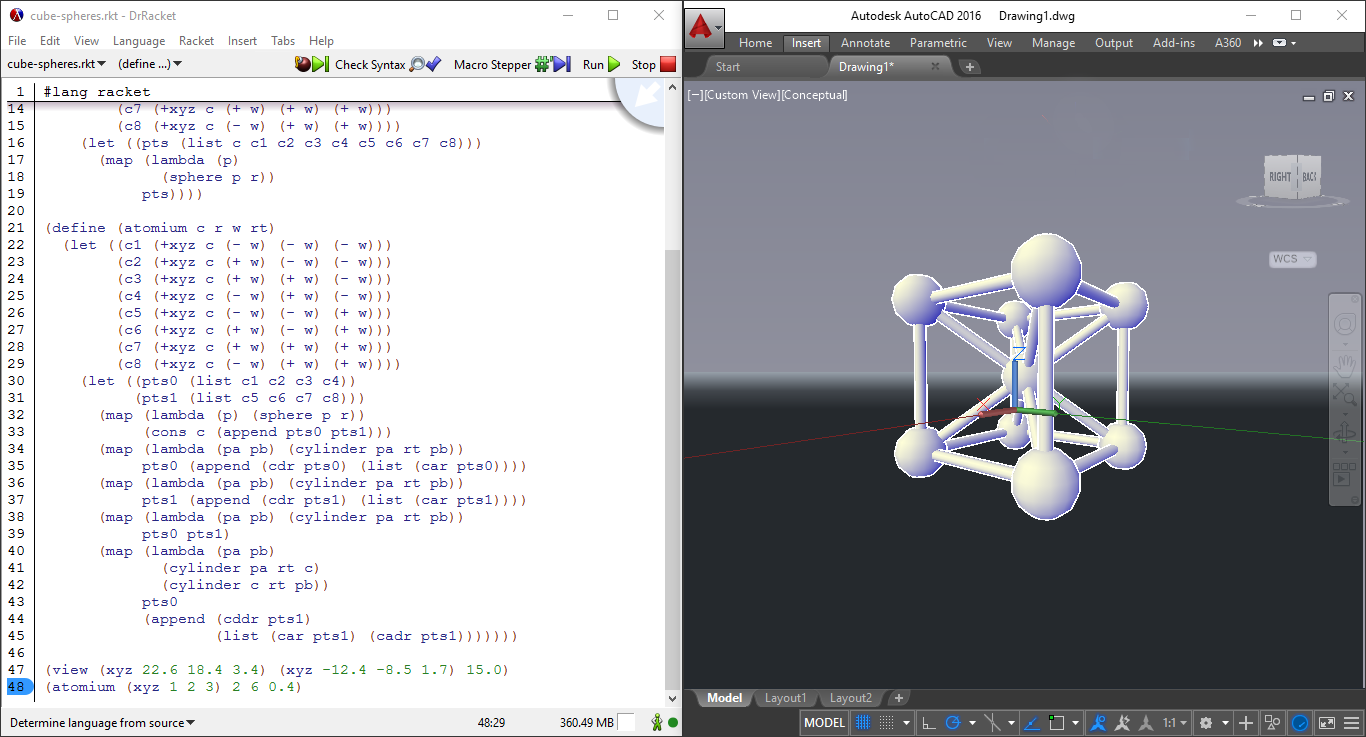
\includegraphics[width=.85\textwidth]{images/rosetta-gui}
    \caption{Rosetta programming system. In the left, is the program written using Racket as the \textit{frontend}. In the right, is the program output using AutoCAD as the \textit{backend}.}
  \label{fig:rosetta-gui}
\end{figure}

Generating the geometric models outside the \gls{cad} application, changes drastically the conventional approach of manually manipulating the \gls{cad} application, making the program a fundamental piece in the design conception. Therefore, facilitate the adherence of novices to this new design paradigm should be a requirement of utmost importance. Rosetta, fortunately, presents a suitable mechanism which serves this purpose. For example, programmers can explore different frontends and backends to find a combination that is most appropriate for the design task. Moreover, programmers have access to various programming languages which can be used interchangeably to write portable \gls{gd} programs. Furthermore, a single program creates identical geometry in different \gls{cad} applications. This approach promotes the development of programs that are portable across the most used \gls{cad} applications, thus facilitating the dissemination of those programs and the underlying ideas. Finally, providing multiple programing languages creates an easy migration path for users of other programming languages, such as, Python and JavaScript, who can find these languages available in Rosetta.

Just as important as being able to choose among multiple frontends/backends is to connect Architects to their design. To this end, many design tools acknowledge the usefulness of immediate feedback. Therefore, this can be seen in the ability of some \gls{gd} tools, such as Grasshopper and Rosetta, to connect program inputs to specialized widgets, such as sliders, that react to changes by recomputing the generated design. However, as discussed in previous sections, this re-computation process only operates in real time for the very simple \gls{gd} program. Sophisticated programs can take a considerable amount of time to recompute, and the interactive use of input widgets can become annoying, a problem that affects any system that depends on \gls{cad} tools for generating geometry.

Because \gls{cad} tools were not designed to process the large volume of operations generated by \gls{gd} program, Rosetta provides an alternative backend that sidesteps most the functionality of traditional \gls{cad} tools and focuses only on generation and visualization of geometric models. This \textit{backend} is based on OpenGL that does not depend on a fully fledged \gls{cad} application. Instead, it connects, almost, directly to the graphics device of the computer. This \textit{backend} allows much faster rendering and, as a result, immediate feedback can operate for larger inputs and a broader spectrum of programs. 

For example, consider the geometric objects shown in Figure~\ref{fig:orto}, Figure~\ref{fig:script}, and Figure~\ref{fig:mobius}. Using a traditional \gls{cad} tool as a \textit{backend}, would be difficult change these objects interactively because to have a fluid feedback the response of an action cannot take more than few seconds (ideally less than 1 second). However, the reaction time of a \gls{cad} application, such as AutoCAD or Rhino, can be very long. 

\begin{figure}[h]
\centering
\begin{minipage}[t]{.33\textwidth}
  \centering
  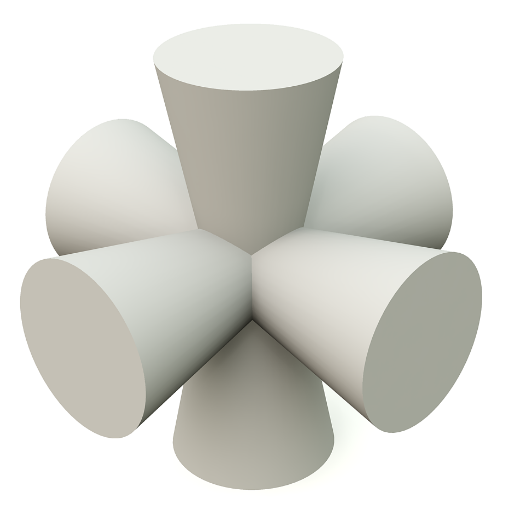
\includegraphics[width=0.8\linewidth]{images/orto-cones}
  \captionof{figure}{Orthogonal Cones}
  \label{fig:orto}
\end{minipage}%
\begin{minipage}[t]{.33\textwidth}
  \centering
  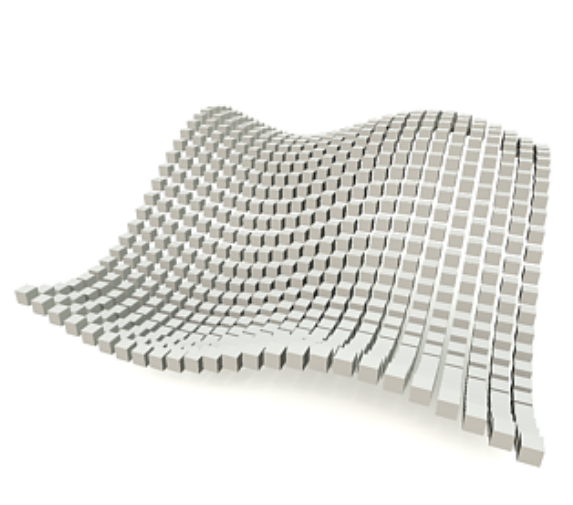
\includegraphics[width=.8\linewidth]{images/scriptecture}
  \captionof{figure}{Scriptecture}
  \label{fig:script}
\end{minipage}
\begin{minipage}[t]{.33\textwidth}
  \centering
  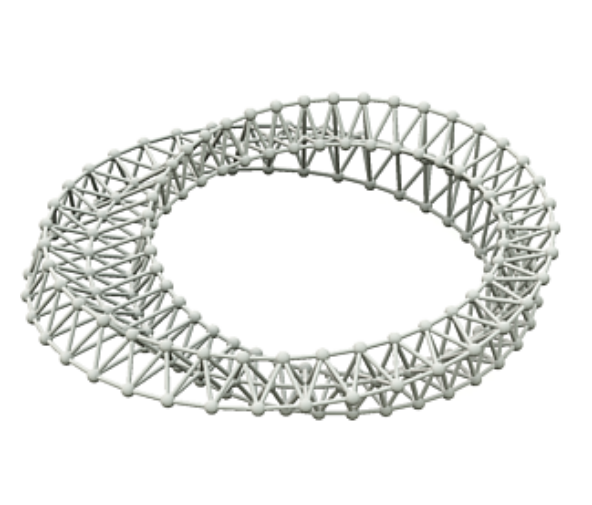
\includegraphics[width=.8\linewidth]{images/truss}
  \captionof{figure}{Möbius Truss}
  \label{fig:mobius}
\end{minipage}
\end{figure}

On the other hand, change these models interactively using the OpenGL \textit{backend} is entirely possible. Table~\ref{tab:runtime} shows the time taken by different backends for updating identical geometry (shown in Figure~\ref{fig:orto}, Figure~\ref{fig:script}, and Figure~\ref{fig:mobius}). It is visible that the OpenGL backend is considerably faster than the other backends. Consequently, an interactive feature that requires immediate feedback will be successful using this backend.

\begin{table}[h]
\centering
\begin{tabular}{@{}lllll@{}}
\cmidrule(r){1-4}
\textbf{Example/Backend} & \textbf{AutoCAD} & \textbf{Rhino} & \textbf{OpenGL} &  \\ \cmidrule(r){1-4}
Orthogonal Cones & 1022 & 191 & 1 &  \\
Scriptecture & 10712 & 2994 & 67 &  \\
Möbius Truss & 24253 & 6094 & 217 &  \\ \cmidrule(r){1-4}
\end{tabular}
\caption{Time (in milliseconds) needed to update the generated geometry}
\label{tab:runtime}
\end{table}

Despite the promising results shown in Table~\ref{tab:runtime}, at this moment, the OpenGL backend is still being developed in Rosetta, and only supports a subset of the functionality that is provided by the other backends. OpenGL is a rendering library. Therefore, it provides several drawing procedures to operate in image space but, in most cases, objects do not have a parametric representation. Thus, this makes it difficult to implement some geometric transformations that \gls{cad} applications provide such as, loft and sweep. Therefore, it is only one of the several challenges to support OpenGL as a backend. However, it is eventually planned to integrate Rosetta.

Finally, the third design principle mentioned provided a strong correlation between programs and models. That means it would be possible for the architect (1) to point to program elements to identify the corresponding model elements, and (2) to point to model elements to determine the corresponding program elements. Fortunately, Rosetta implements a traceability mechanism. Therefore, designers can use both approaches at the same time, moving from one to the other as necessary, thus accelerating the development process.

For example, Figure~\ref{fig:program-shape} illustrates a typical scenario where the user selects an expression in his program and
Rosetta shows the set of shapes that resulted from that expression. Note that this set contains all shapes that were created by the expression during the complete execution of the program. Figure~\ref{fig:shape-program} illustrates the inverse scenario, in which a user selects an element of the model in the \gls{cad} application and Rosetta highlights the corresponding program elements and control flow.

\begin{figure}[h]
  \centering
  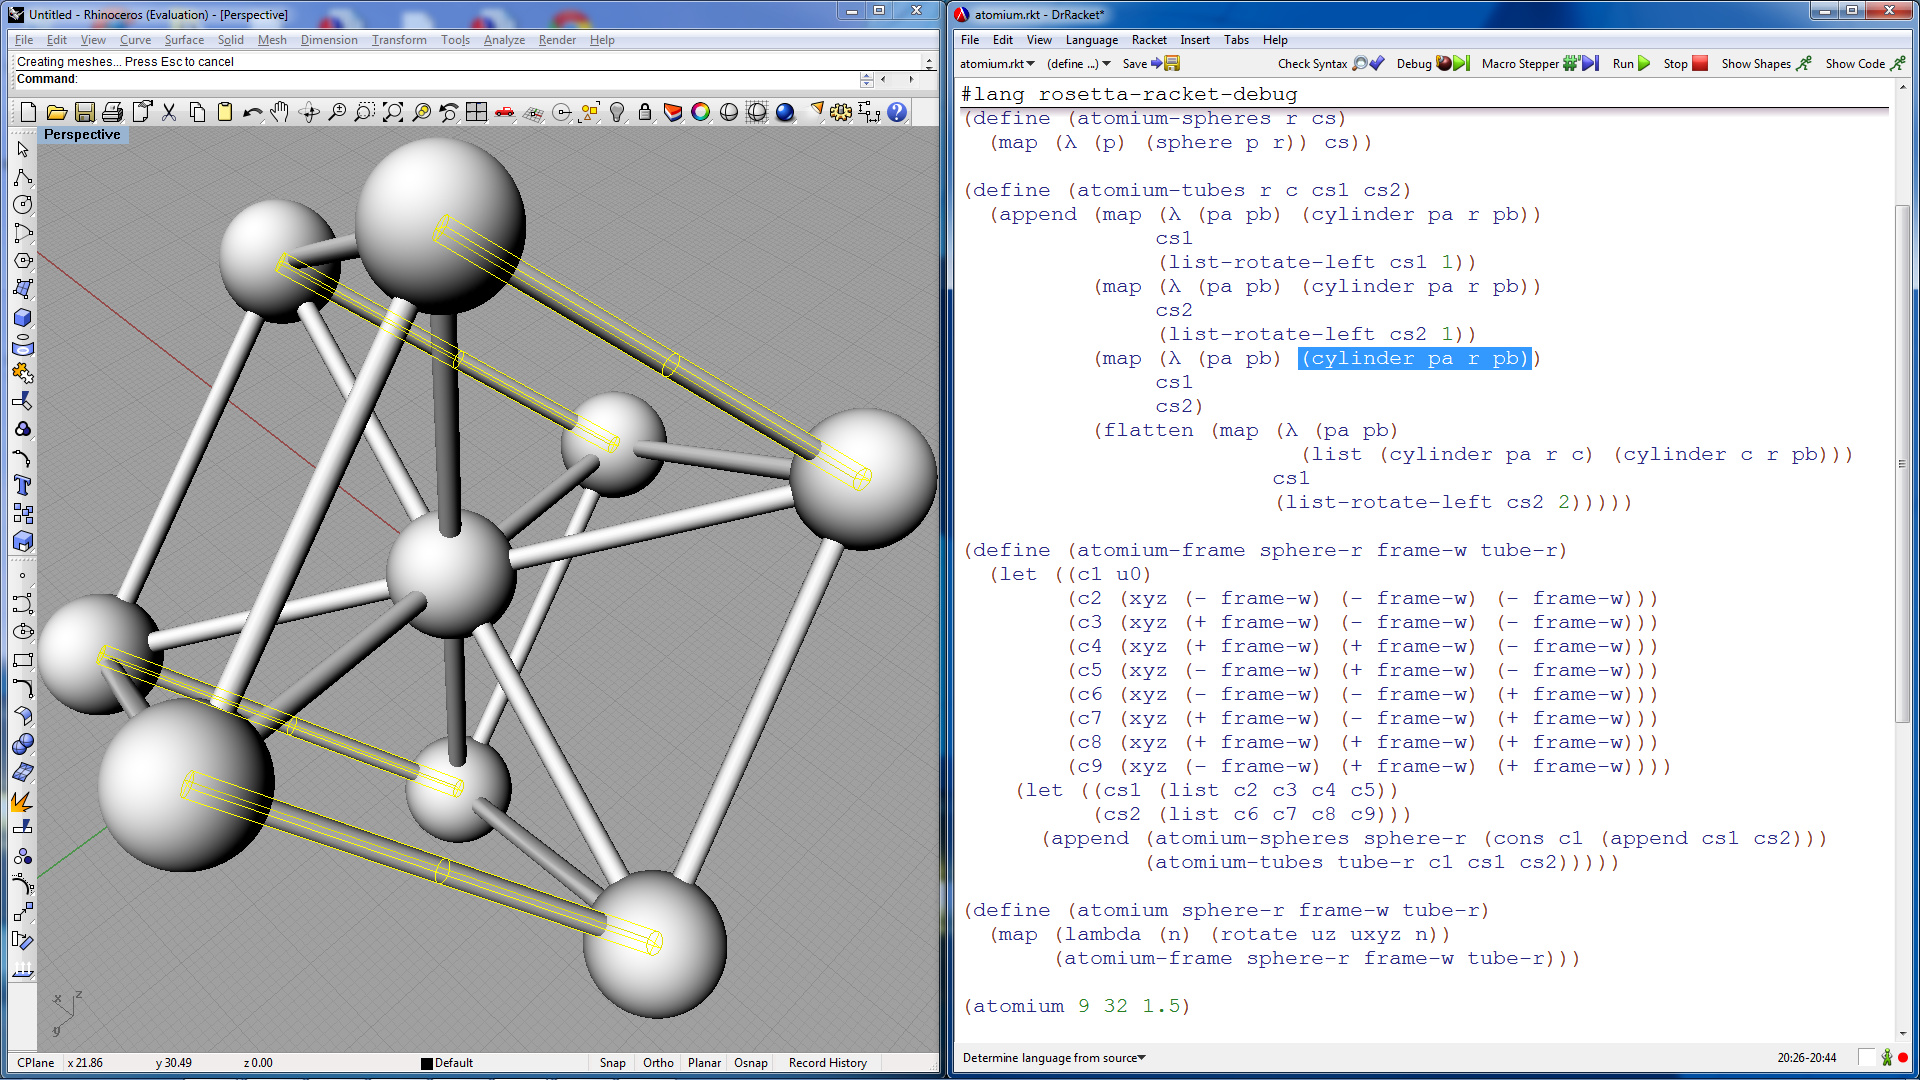
\includegraphics[width=.85\textwidth]{images/program-to-shape}
    \caption{Rosetta traceability tool, relating program expressions to the generated shapes. The highlighted cylinders (on the left, in yellow) are produced by the highlighted expression (on the right, in blue).}
  \label{fig:program-shape}
\end{figure}

\begin{figure}[!htbp]
  \centering
  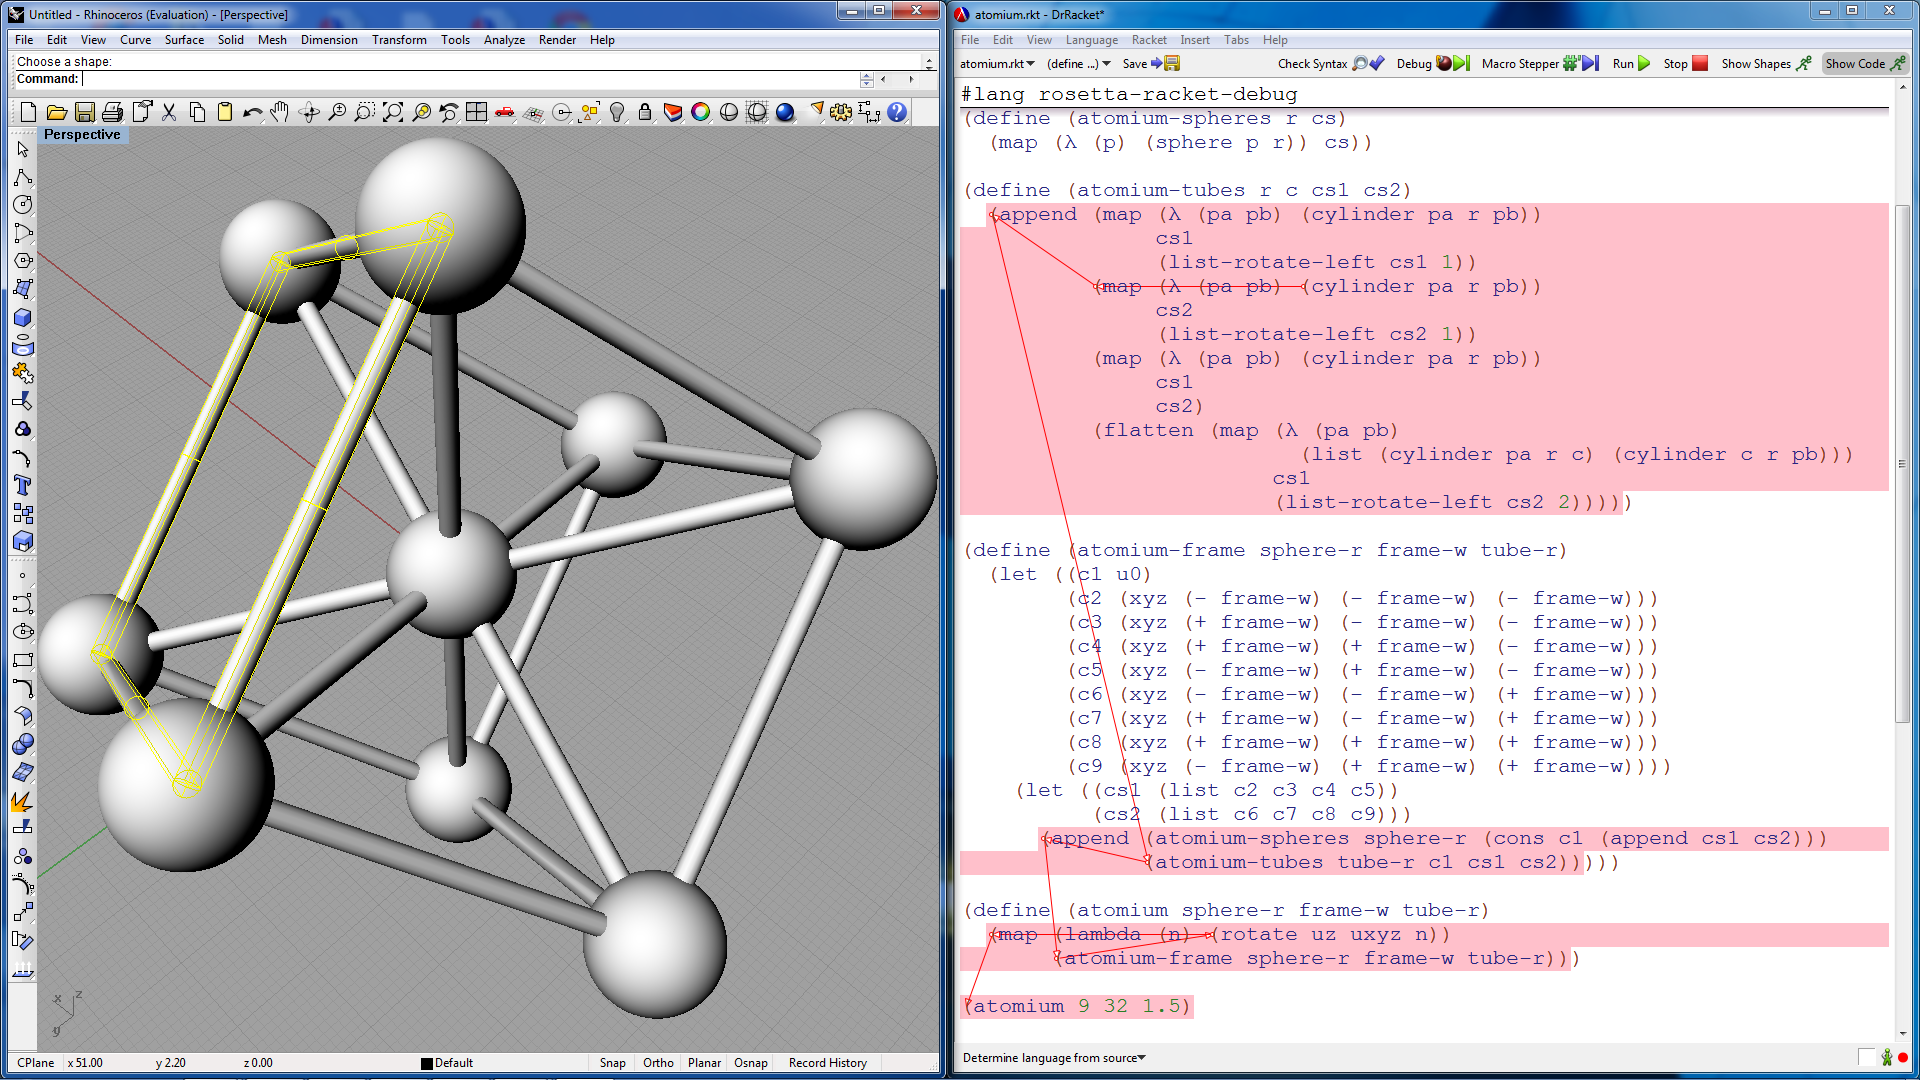
\includegraphics[width=0.85\textwidth]{images/shape-to-program}
    \caption{Rosetta traceability tool, relating shapes to the program expressions that generated them. The highlighted program flow makes the highlighted cylinders (on the left, in yellow) (on the right, using red arrows).}
  \label{fig:shape-program}
\end{figure}

The main advantage of using Rosetta as a pillar of development is that all these features are given to the programmers, as a "package", without any apparent effort. However, we are confined to use the current programming environment used in Rosetta: DrRacket. In the next section, I present relevant properties of this environment that can benefit the implementation. 

\section{DrRacket}

DrRacket, shown in Figure~\ref{fig:drracket-gui}, is a programming environment designed to be pedagogic and to simplify the implementation of new programming languages and tools. It provides a text editor with the standard programming features, such as text formatting, and syntax checking and highlighting. Programs are written in the Definitions Window and the Run button, in the Tool Bar, compiles the program and its dependencies and initiates its execution. During execution, the Interactions Window becomes available, providing an interactive evaluator which can be used to test the running program quickly, add new definitions to the session, experiment with different parameters or, ultimately, evaluate any expression. This evaluator is fundamental for incremental development and interactive testing, being one of the primary sources of feedback during program development.

\begin{figure}[!htbp]
  \centering
  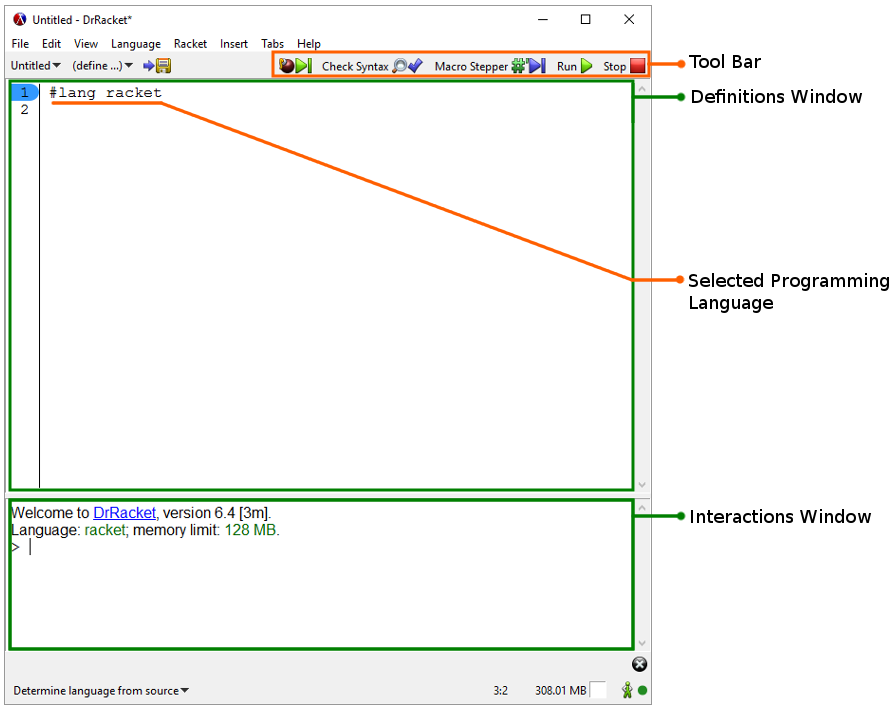
\includegraphics[width=0.75\textwidth]{images/drracket-gui}
    \caption{DrRacket programming environment, showing Definitions Window and Interactions Window (in green) where users write and evaluate their code, and (in orange) the selected programming language and the toolbar menu.}
  \label{fig:drracket-gui}
\end{figure}

Despite the DrRacket properties listed above, to choose DrRacket as implementation base, we on these three main features:

\begin{itemize}
    \item \textbf{Pedagogic.} DrRacket is widely used in introductory courses for programming languages. Its environment is designed to guide the student by catching typical mistakes and explaining them in terms that students understand. It is also useful for professional programmers, due to its sophisticated programming tools, such as the static debugger, and its advanced language features, such as \textit{units} and \textit{mixins}.

    \item \textbf{Sophisticated editor.} DrRacket fully integrates a graphics-enriched editor which supports, in addition to plain text, elements such as images and boxes (with comments, Racket code or XML code). DrRacket also displays these elements appropriately in its read-eval-print loop.

    \item \textbf{Extensible.} The main tools of the DrRacket environment are implemented using the same \gls{api} that is available for extension. For example, the debugger, the syntax checker, and the stepper, despite providing different functionalities, are implemented on top of the same \gls{api}.
\end{itemize}

Finally, DrRacket helps programmers to understand the syntactic and lexical structure of their programs, because it provides a syntax checker that annotates a syntactically correct program in five categories (1) primitives, (2) keywords, (3) bound variables, (4) free variables, and (5) constants. When the programmer moves the mouse over an annotated identifier, the syntax checker displays graphical arrows that point from bound identifiers to their binding occurrence, and vice-versa. However, the syntax checker ignores the category of comments, including its visual elements such as the images. As a result, these items are uncorrelated with the program's structures and behavior.

\section{Implementing the proposed tools}

The problem addressed in this thesis is to design and implement an interactive programming environment for generative design that covers the needs of \gls{gd} community. The approach described in Chapter~\ref{chapter:pegd}, suggests two interactive tools: (1) \textit{program-sketch correlation tool}, which correlates sketches with code, as a result, it significantly reduces the effort to read the code, and (2) \textit{immediate feedback tool}, which executes the program upon changes, thereby creating an interactive environment to users quickly test their ideas and, eventually, improve their program comprehension.

\subsection{Program-sketch correlation tool}
\label{sec:psct}

There are two ways to correlate a generative design program with its produced model. The first is using a sketch in the program that illustrates the intended model. The second is using the generated model, correlating the elements of the shape with fragments of the code. The first type of correlation did not exist in Rosetta, consequently this is a contribution of this thesis.

The \textbf{program-sketch correlation tool} was implemented using the power of DrRacket syntax check to bind annotated identifiers. In this way, the images resources, already supported in the text editor, now becomes a new category of rich-media expressions included in the syntax check annotated types. As a result, programmers can add in their functions, images that illustrate the purpose of that function. Therefore, this is perfectly suitable for functions used in \gls{gd} programs, because usually the output of these functions can be visually represented by a sketch.

For example, Figure~\ref{fig:rmeaning} shows a typical example where the architect defines a function that creates a cube with spheres in its vertices. In this example, the architect can start by searching for each function argument, moving the mouse over them, to find the meaning of these arguments in code. Inversely, as shown in Figure~\ref{fig:figmeaning}, he can start from the image by moving the mouse over it, to find the meaning of these arguments in code. Furthermore, programmers can use images in their programs, and the image inserted in the function body acts as if it was part of the program. However, internally it continues to be a mere code comment that does not affect the correct operation of the function.    

\begin{figure}[!h]
\centering
\begin{minipage}[t]{.495\textwidth}
  \centering
  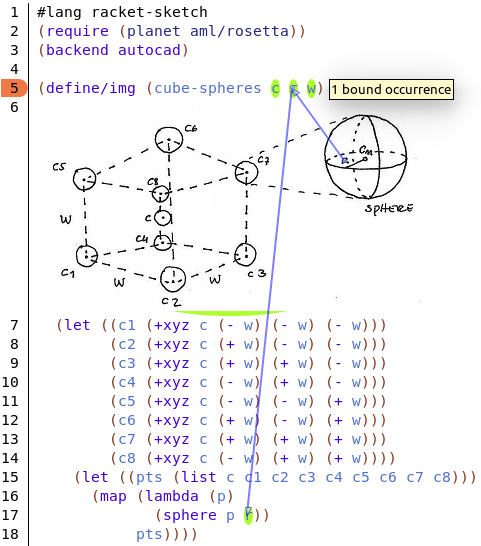
\includegraphics[width=1\linewidth]{images/img-code}
  \captionof{figure}{Relating function arguments with image. The highlighted argument (under the cursor, in green) is illustrated in the image (on the \texttt{R} symbol, using blue arrows).}
  \label{fig:rmeaning}
\end{minipage}%
~
~
\begin{minipage}[t]{.495\textwidth}
  \centering
  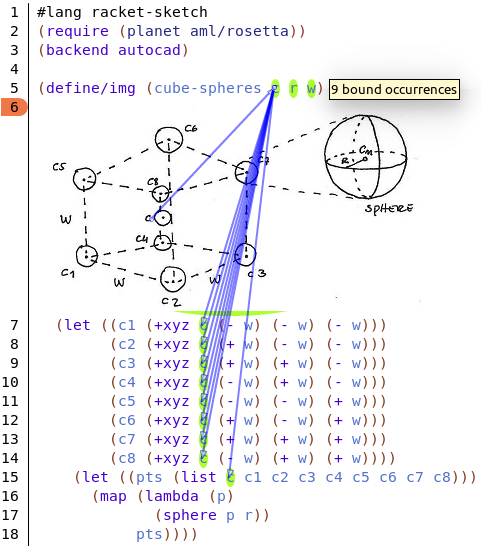
\includegraphics[width=1\linewidth]{images/img-code-2}
  \captionof{figure}{Relating image with function arguments. The parameter illustrated in the image (on the \texttt{c} symbol, under the cursor) is highlighted in the code (in green, using blue arrows).}
  \label{fig:figmeaning}
\end{minipage}
\end{figure}

Although images are a suitable media to represent geometric objects, textual information can also be appropriate in some cases. For example, 
during the development of the program, usually, several functions are created. Consequently, the architect may not have a sketch to document them. Furthermore, the process to draw a new sketch, import it to the computer, and insert it in the code, is clearly more laborious than writing a simple piece of text that describes the function. Using this method he can later complete his code with a proper sketch, but until then the function is still documented, and he can share his code without any trouble.

Thinking about this situation, I extended the program-sketch correlation tool to support also source code comments. Similarly to the correlation with images, users can insert a string that explains the method. This string can be annotated with special characters to correlate its characters graphically to the function identifiers. For example, Figure~\ref{fig:ortocone1} portrays a typical situation where the architect is reading the function comment and moves the mouse over an annotated identifier (\texttt{@orthogonal-cones}). Thus, immediately, some arrows are displayed that point to the definition of that function, and also to its use in the program context. Figure~\ref{fig:ortocone2} shows a different situation where the architect points to a function parameter and some arrows are displayed to the use of that parameter, including to its explanation in the code comment. 

\begin{figure}[!h]
\centering
\begin{minipage}[t]{.495\textwidth}
  \centering
  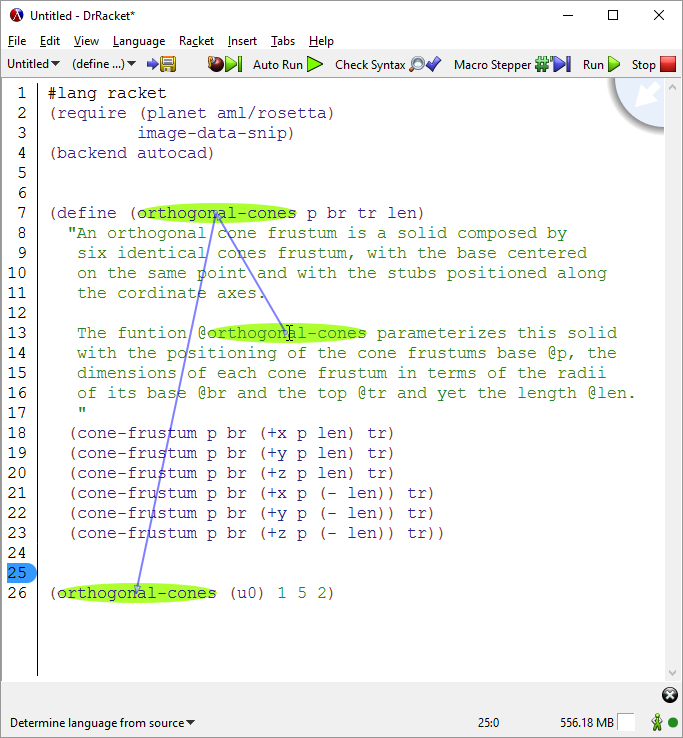
\includegraphics[width=1\linewidth]{images/orto-cone-1}
  \captionof{figure}{Relating code comments with function arguments. The highlighted function name (under the cursor, in green) is linked to its definition and utilization in the source code (in green, using blue arrows).}
  \label{fig:ortocone1}
\end{minipage}%
~
~
\begin{minipage}[t]{.495\textwidth}
  \centering
  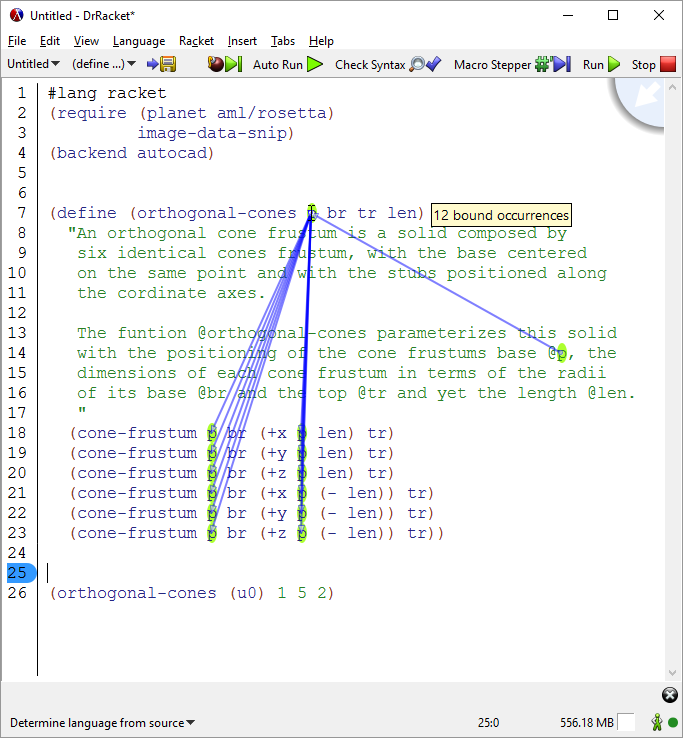
\includegraphics[width=1\linewidth]{images/orto-cone-2}
  \captionof{figure}{Relating function arguments with code comments. The highlighted function parameter (under the cursor, in green) is linked to its utilization in the code comment (in green, using blue arrows).}
  \label{fig:ortocone2}
\end{minipage}
\end{figure}

Regarding the usability of this tool, an inherent concern already noted is related to the use of images in the text editor. As shown in Figure~\ref{fig:expanded}, images may have arbitrary dimensions and may occupy large areas of the text editor, which may cause bad experiences in the utilization of this tool, affecting the readability of the code, and, even worse, disturbing the user in his primary task: programming.

To avoid this problem, I propose a straightforward mechanism that allows collapsing the images. As a result, images are reduced to the height of a character sentence, using considerably less space than before (e.g. see Figure~\ref{fig:collapsed}). Once the picture is collapsed the programmer can easily navigate through the code, improving his awareness of the surrounding context in a file. Furthermore, this feature can be enhanced by DrRacket collapse \textit{S-expressions tool} to elide code. However, differently from moderns code editors that collapse the code in blocks, when the architect wants to view part of the surrounding context, he either have to over the collapsed code to show a tool tip, possibly occluding relevant code, or expand the collapsed code possibly moving relevant code off-screen. DrRacket omits code by replacing it with "\texttt{(...)}", this way the surrounding context is still legible but uses less space. Inversely, users can expand their code as well as their images by a simple click. Note that all information placed in the picture, i.e. the annotated positions where the arrows will point, continue as before. However, when an image is collapsed this change is not persisted in the stored file, it just sets the dimensions ports of the window visualization. Consequently, the programmer needs to perform this operation every time he starts a new session. 

\begin{figure}[!h]
\centering
\begin{minipage}[t]{.495\textwidth}
  \centering
  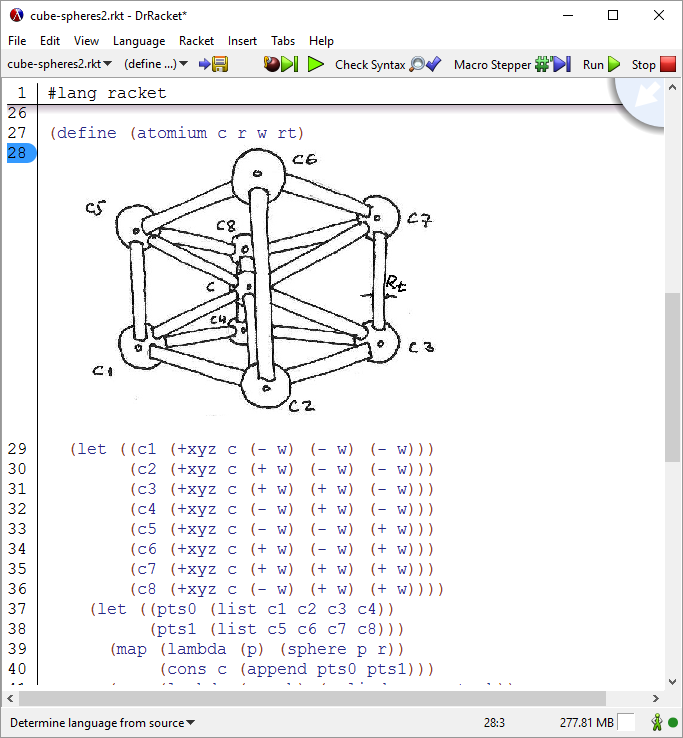
\includegraphics[width=1\linewidth]{images/atomium-expanded}
  \captionof{figure}{Inserting in the text editor an image with large dimensions. The function body is separated from its head definition due the large dimensions occupied by the image.}
  \label{fig:expanded}
\end{minipage}%
~
~
\begin{minipage}[t]{.495\textwidth}
  \centering
  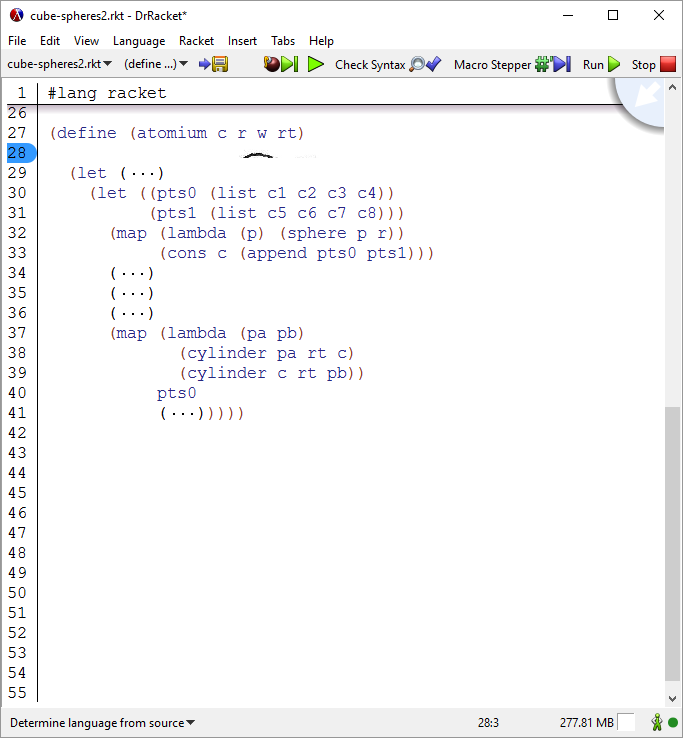
\includegraphics[width=1\linewidth]{images/atomium-collapsed}
  \captionof{figure}{Collapsing the image and some s-expressions. The code is collapsed, tidy, and the surrounding context is still legible.}
  \label{fig:collapsed}
\end{minipage}
\end{figure}


In order to automatically recognize symbols in images and binding them with code identifiers, the presented architecture, in Chapter~\ref{chapter:pegd}, suggested the use of an \gls{ocr} engine. Thus, the \gls{ocr} engine is intended to receive the images, process their optical characters, and return the characters found with their respective coordinates on the picture. The first approach taken followed this description, sending the sketches, such as the one shown in Figure~\ref{fig:rmeaning}, to the \gls{ocr}. Unfortunately, this process was unfruitful, mainly because the technologies used in the current \gls{ocr} engines have several problems to identify handwritten symbols (especially in the case of mathematical annotations) and they fail to recognize correctly the symbols used in the sketches in (almost) 100\% of the times.

However, to finish the implementation of this tool without depending on the correct functioning of the \gls{ocr} engine, I implemented a \textit{fallback} mechanism that allows users to perform the \gls{ocr} work. This way, when the first image of a function body is inserted in the code editor, it is blindly annotated with the same position for all function parameters. As a result, DrRacket check syntax will draw binding arrows, from the center of the image, to the function arguments, and vice-versa. For example, Figure~\ref{fig:init-state} shows precisely this moment, after the picture is inserted in the function body. At this point, it is up to the programmer to change the bind position of each parameter to the correct position; the tool does not require this action. 

\begin{figure}[!h]
\centering
\begin{minipage}[t]{.495\textwidth}
  \centering
  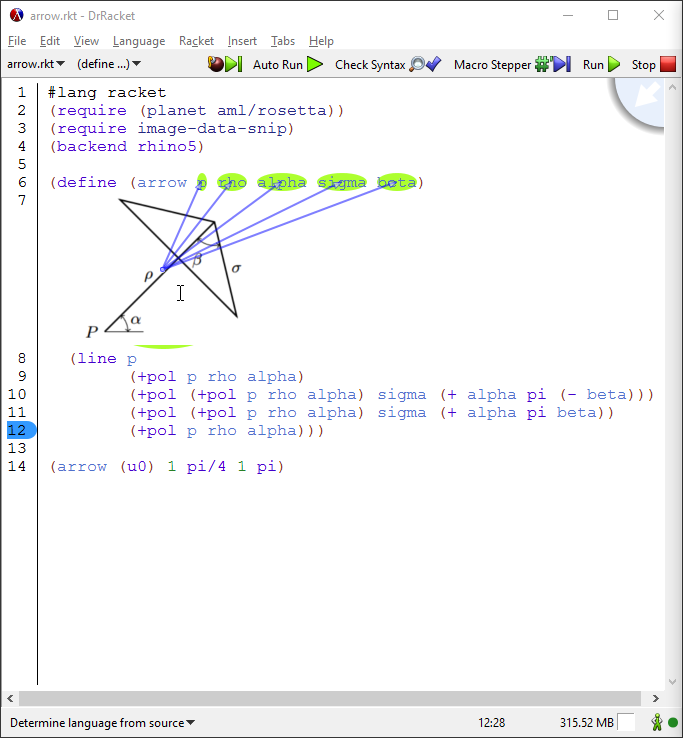
\includegraphics[width=1\linewidth]{images/1}
  \captionof{figure}{After inserting, in the text editor, the first image to illustrate the function parameters. The arrows (in blue) come from the center of the image (under the cursor) to the  highlighted parameters (in green).}
  \label{fig:init-state}
\end{minipage}%
~
~
\begin{minipage}[t]{.495\textwidth}
  \centering
  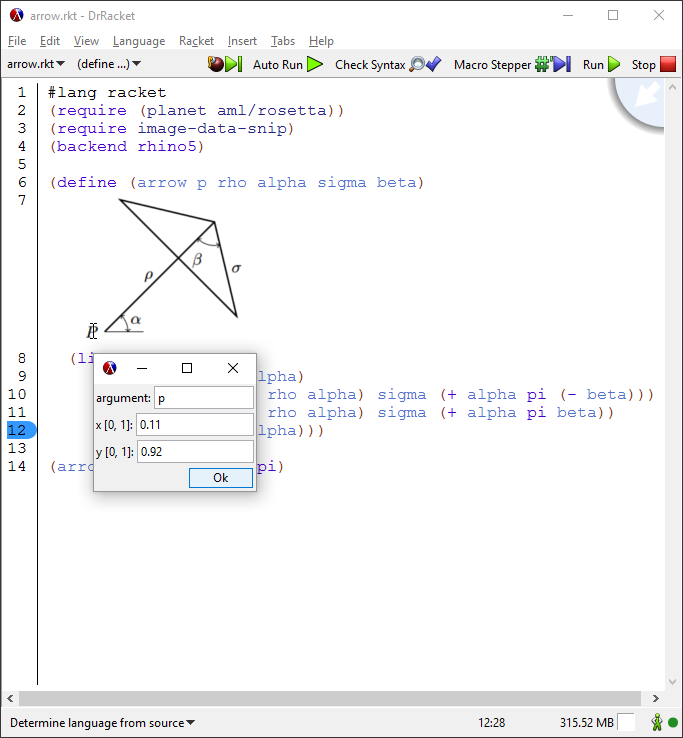
\includegraphics[width=1\linewidth]{images/2}
  \captionof{figure}{Choosing the correct position for the function parameter \texttt{p}. The coordinates of the point \texttt{p} (illustrated in the image) as well as its correspondent function parameter is shown in the \gls{gui}.}
\label{fig:gui-set-param}
\end{minipage}
\end{figure}

\begin{figure}[!h]
\centering
\begin{minipage}[t]{.495\textwidth}
  \centering
  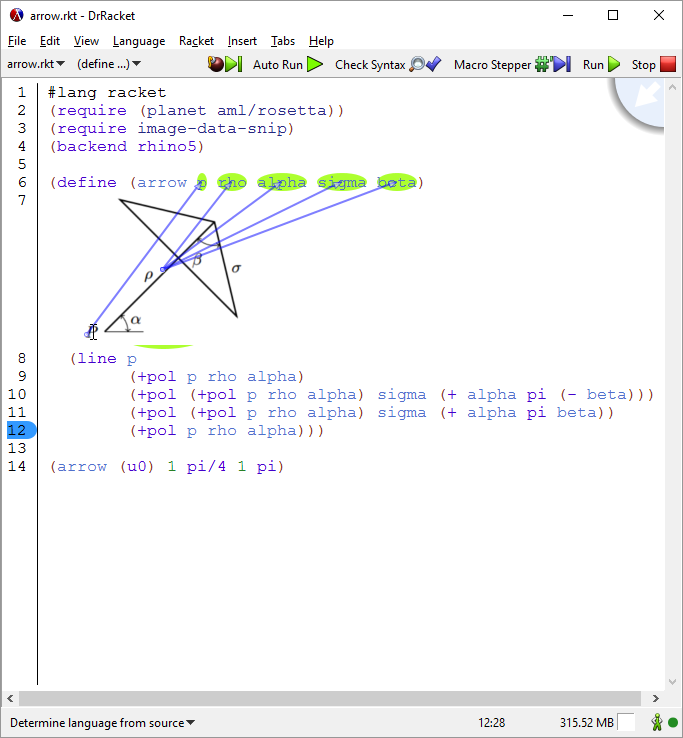
\includegraphics[width=1\linewidth]{images/3}
  \captionof{figure}{Showing the correct binding association of the parameter \texttt{p}.}
  \label{fig:one-right}
\end{minipage}%
~
~
\begin{minipage}[t]{.495\textwidth}
  \centering
  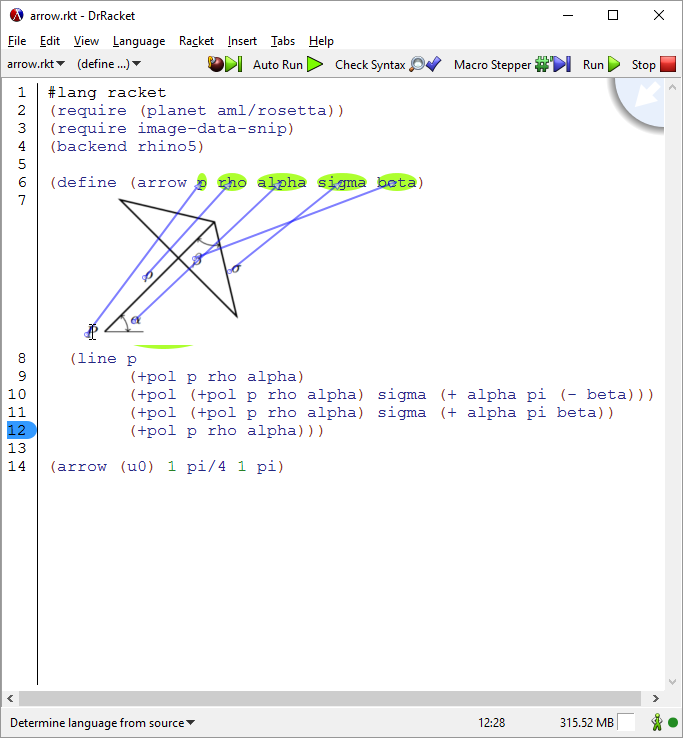
\includegraphics[width=1\linewidth]{images/4}
  \captionof{figure}{Finishing the process setting all the image symbols in their proper place.}
  \label{fig:alright}
\end{minipage}
\end{figure}

Further, to finalize this process and have the right associations between image symbols and function identifiers, an alternative method was implemented. So, if the programmer clicks in any space of the picture, a \gls{gui} will appear showing three fields: (1) the \texttt{parameter} field, that is empty by default, and it is intended to specify the name of the clicked symbol, which, of course, must match with the function parameter name; (2) the \texttt{x}; and (3) the \texttt{y} fields, that defines the width and height of the coordinate respectively. These areas are filled by default with the clicked position got from the image space. However if the user wants to specify another value, it is also possible.

Figure~\ref{fig:one-right} shows the effect of setting a single function parameter using this method. As we can see, the other parameters stay in the same position. Moreover, to correct the others associations the programmer must repeat this process for each parameter. For example, Figure~\ref{fig:alright} shows the final result where all parameter is correctly identified. As a result, DrRacket can draw arrows directly to each one of them. Note that; this process is only performed once because the information associated with the image is stored with the source code file.

\subsection{Immediate feedback tool}

As discussed previously, despite the apparent advantages of using a \gls{gd} approach to model geometric objects, this method presents, at least, one important drawback that affects the design process. Architects cannot interact with their models as they build it. Any change in the model must be performed first in the code, and only after the program is compiled and executed the alterations will be available on the model. This process apparently takes more time than the traditional approach of manually building the model in the \gls{cad} tool. Besides, it discourages the artistic work because the changes are more costly than just manipulating a \gls{gui} element.

In Chapter~\ref{chapter:pegd} we suggested the \textbf{Immediate feedback tool} that aims to overcome this limitation, trying to promote the creative work in the design phase. This tool seeks to reduce as much as possible the time between a change in the code and its visualization in the model. Several techniques were suggested particularly considering the current state of \gls{gd} environments.

Regarding some of these proposed methods, and trying to put them in practice, I implemented the immediate feedback tool on top of DrRacket. Once DrRacket is the programming environment used by Rosetta, any improvement achieved in this programming environment will be useful for both systems. So, I started by extending the current DrRacket environment developing an external tool, i.e. a \textit{\textit{plugin}}. The \textit{\textit{plugin}} was used to access the DrRacket \gls{api} without having to modify it.

Therefore, to use this tool users can install it separately, and uninstall it at any time. Once the tool is installed, a new icon will appear on the top of DrRacket Tool Bar. This icon has a symbol (similar to the DrRacket Run icon) and a description. However it has a responsive behavior: if the DrRacket window is too small the description will be omitted to save space and maintain the interface cohesive. When the user clicks on it, its color changes meaning that it is in action. Immediately after clicking, apparently nothing will occur until an expression is ready for evaluation.

\begin{figure}[!h]
\centering
\begin{minipage}[t]{.495\textwidth}
  \centering
  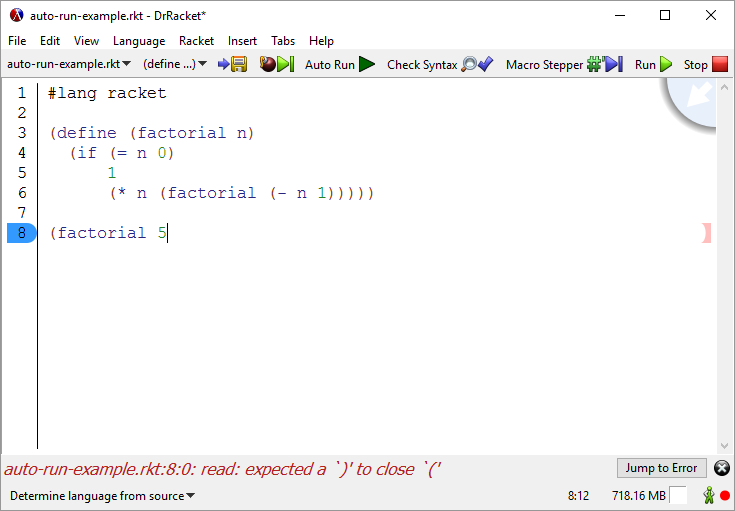
\includegraphics[width=1\linewidth]{images/fact}
  \captionof{figure}{Using the Auto Run tool (in dark green) when writing the factorial function. The highlighted expression is incomplete.}
  \label{fig:fact-incomplete}
\end{minipage}%
~
~
\begin{minipage}[t]{.495\textwidth}
  \centering
  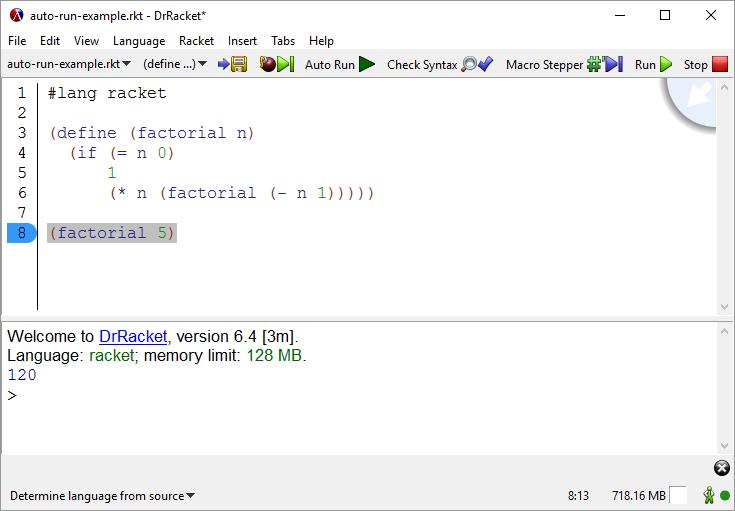
\includegraphics[width=1\linewidth]{images/fact-eval}
  \captionof{figure}{Immediately after closing the right bracket of the highlighted expression. The Interactions Window is shown with the function result.}
  \label{fig:fact-complete}
\end{minipage}
\end{figure}


For example, Figure~\ref{fig:fact-incomplete} shows an example where the \textit{Auto Run tool} is activated and the programmer is writing the factorial function. At each character insertion, this tools is desperately trying to execute the code. However, to perform this action, the code needs to be syntactically correct. On the other hand, the Check Syntax is validating the code, catching any syntax error and showing them at the bottom bar. Furthermore, when Check Syntax finishes its validation, and the code is syntactically correct, the AutoRun tool can operate. So it gets all the code validated previously, creates a callback, and sends it to the DrRacket evaluator. As a result, the code is immediately executed, as shown in Figure~\ref{fig:fact-complete}.

Unlike the factorial function that returns a numeric output, the functions in \gls{gd} return a visual object. In this context, this tool is even more useful, because the changes made in the code causes a visual effect in the geometric object. The combination of this technique with the generated objects can provide an interactive environment, to experiment new ideas and test parametric models quickly.

However, the experimentation of program inputs relies heavily on the keyboard, breaking the fluidity of this process. For this, I used the DrRacet a widget mechanism to provide sliders at the program input. Thus, users can drag the slider to change the program input, rather than delete and insert a new character. Each shift in the slider causes an execution of the program with the new slider value. In \gls{gd} programs this will generate a new geometric model. As a result, users can check if that value created the desired shape. 

\begin{figure}[!h]
  \centering
  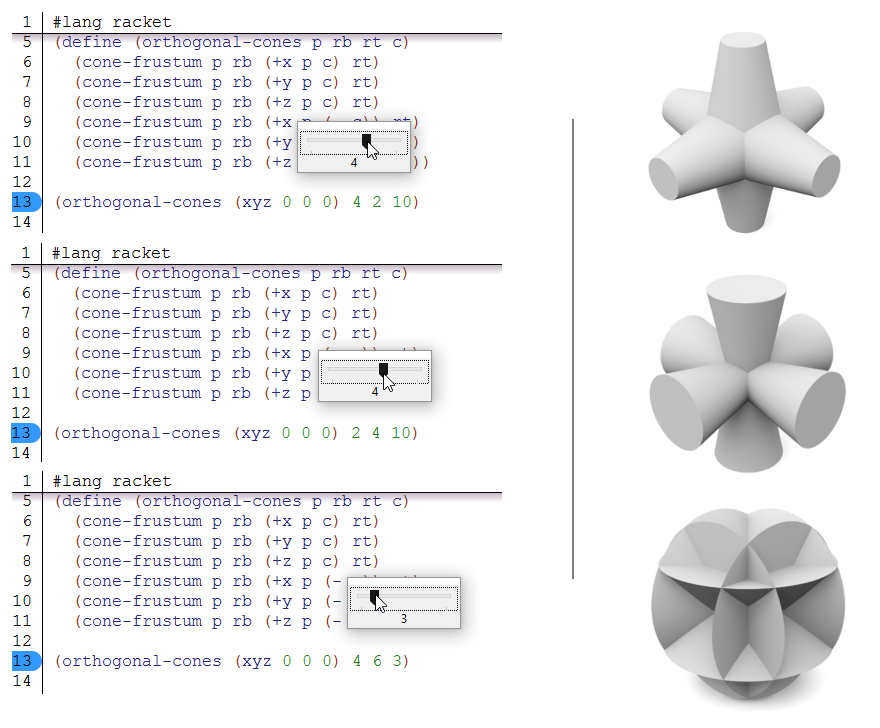
\includegraphics[width=.8\textwidth]{images/orto-cones-run}
    \caption{Using the slider widget with \textit{Auto Run tool} active, to experiment some input values. The highlighted function call (at line 13, on the left) is being changed by the slider (over the pointer). On the right, are the generated shapes rendered by AutoCAD.}
  \label{fig:orto-cone-run}
\end{figure}

Figure~\ref{fig:orto-cone-run}, shows the use of this tool to generate some geometric shapes. Despite the notable difference among the created forms, the function used to produce them is the same (this function is also shown in Figure~\ref{fig:ortocone1}). Therefore, the programmer can experiment several input values by just dragging the slider, once he achieved an intended design he can copy that line of execution (as a code comment for instance) and continue to experiment other values. The slider appears on top of a selected input number, to facilitate this process. It has a compressed window without any extra buttons, as a way to be integrated with the text editor. Thus, users only need to click back into the text editor to close this window and be back to edit code.

Regarding the usability of this tool, the faster will be the backend response as better will be the user's experience. For example, consider the function \texttt{orthogonal-cones} (shown in Figure~\ref{fig:ortocone1}), its execution time is relatively straightforward (e.g. in AutoCAD backend it takes approx. 1  second, as shown in Table~\ref{tab:runtime}). This is a tolerable delay between a model update, however using a more compounded geometry, such as the Möbius Truss, in Figure~\ref{fig:mobius}, or even a complex geometry, such as a building, the execution time can grow considerably, and the immediate feedback becomes almost impossible. 

% \begin{figure}[h]
% \centering
% \begin{minipage}[t]{.65\textwidth}
%   \centering
%   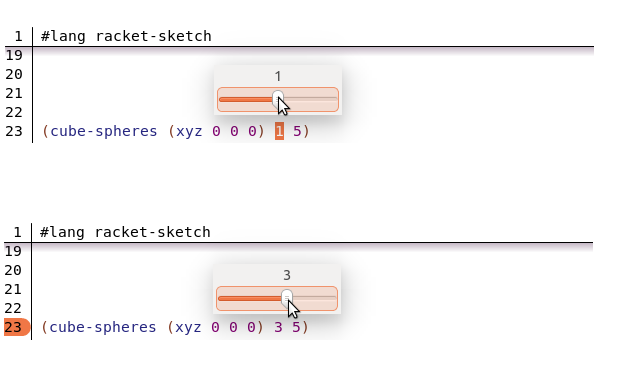
\includegraphics[width=1\linewidth]{images/cube}
%   \captionof{figure}{Relating function arguments with image. The highlighted argument (under the cursor, in green) are illustrated in the image (on the \texttt{R} symbol, using blue arrows).}
%   \label{fig:img-cube1}
% \end{minipage}%
% ~
% ~
% \begin{minipage}[t]{.35\textwidth}
%   \centering
%   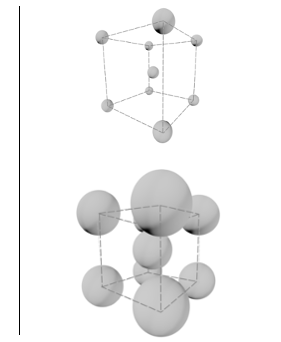
\includegraphics[width=1\linewidth]{images/img-cube}
%   \captionof{figure}{Relating image with function arguments. The parameter illustrated in the image (on the \texttt{c} symbol, under the cursor) are highlighted in the code (in green, using blue arrows).}
%   \label{fig:img-cube2}
% \end{minipage}
% \end{figure}


\section{Implementation Details}

\subsection{General architecture}

Figure~\ref{fig:solution} presents the general architecture of the solution, in a publish-subscribe view. There are two different interactions in this architecture, the first presented by a publish-subscribe, and the second by a client-server.

\begin{enumerate}
    \item The main functionality of the proposed environment is made through a publish-subscribe interaction. The \texttt{DrRacket \gls{ui} event manager} acts as an event bus for user-interface events (such as button clicks, character insertion, etc.). From this event bus, I subscribe only the \gls{ui} events which are relevant to the system, defining which components will handle them. It is done at load time when the event manager reads the \textit{\textit{plugin}} configuration file (i.e. \texttt{info} file). When users are working on the editor, an \gls{ui} event is generated and dispatched via implicit invocation to the action handler objects that subscribe to that event.

    \item Despite the presented solution does not include the automatic character recognition, this module is part of the planned architecture, and can be considered, for a future integration. Thus, a client-server interaction will be needed to automatically recognize the manuscript symbols present in the image, using to this end an external \gls{ocr} engine. Thereby in the suggested architecture the \texttt{symbol identifier} component calls this service to handle the recognition of symbols in the image. However, in the implemented architecture this component generates by itself the \gls{ocr} data and all other modules continue to work as before.  
\end{enumerate}

\begin{figure}[htb]
    \centering
    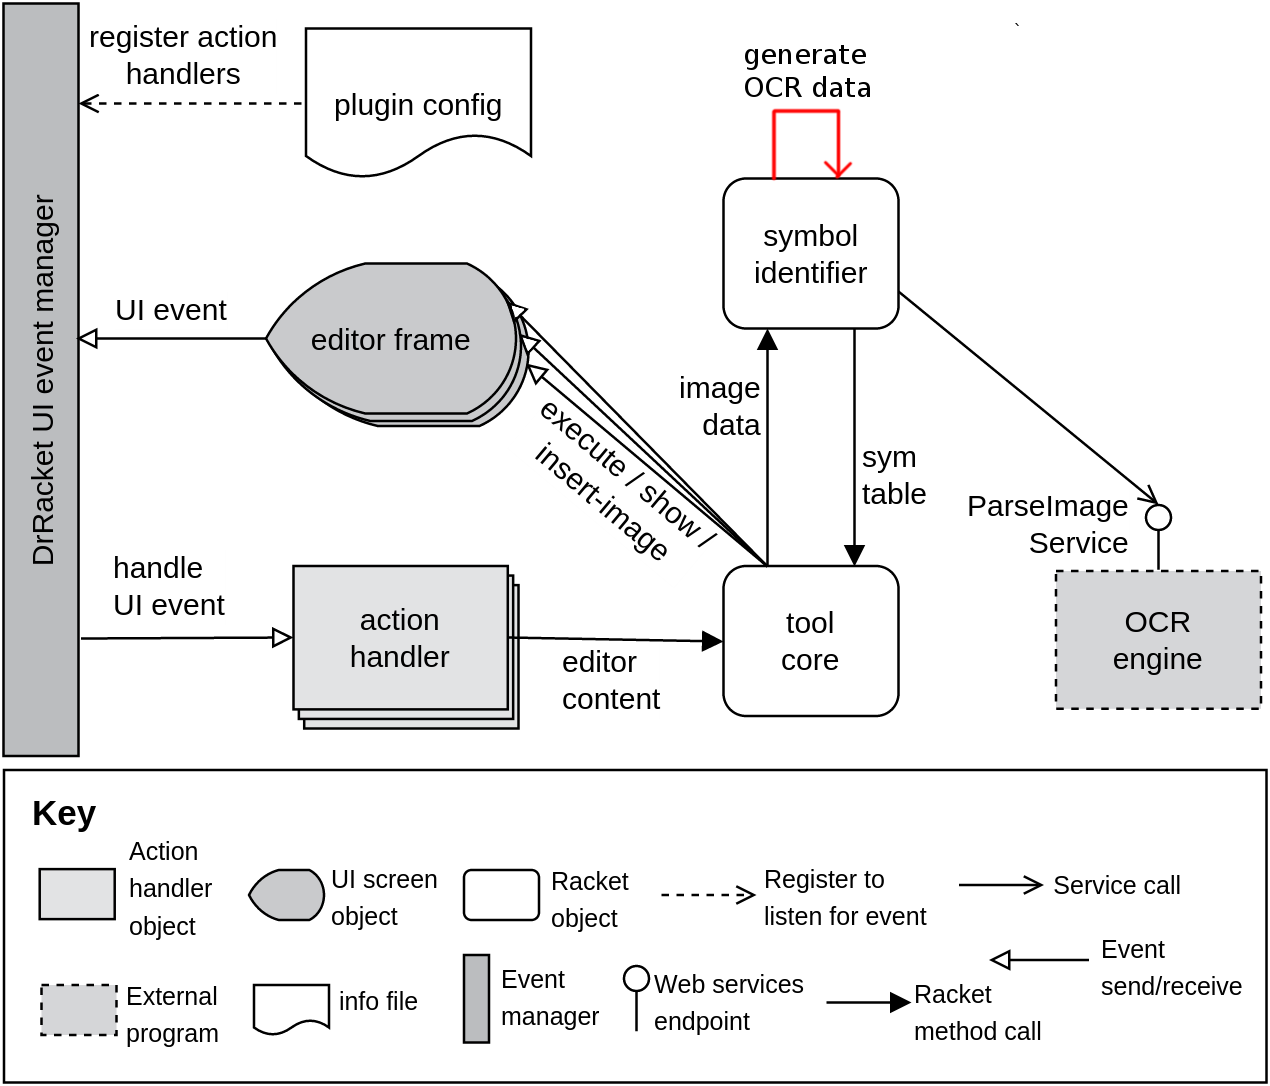
\includegraphics[scale=0.22]{images/solution}
    \caption{Diagram for a publish subscribe view of the proposed architecture. The arrow, in red, on top of the \texttt{symbol identifier} module shows the implemented architecture.}
    \label{fig:solution}
\end{figure}

The \texttt{tool core} component, in Figure~\ref{fig:solution}, receives, three relevant kinds of DrRacket events. For each of these events, the programming environment is changed executing the following actions:

\begin{itemize}
    \item \texttt{on-change:} when DrRacket detects that the editor has been modified, it sends the contents of the editor over to action handlers.    In this case, it sends this information to the \texttt{online expansion handler} where the code is expanded. \textit{Executed action}: sends a \texttt{execute} event to the editor frame, if the action handler expanded the code successfully. 

    \item \texttt{on-paint:} this event is sent just before and just after every element is displayed in the editor. Handling this event provides a way to add arbitrary graphics to the editor screen. \textit{Executed action}: sends a \texttt{show} event to the editor frame, to display a slider widget when the user presses the mouse over a literal.

    \item \texttt{on-new-image-snip:} this event is sent when an image is inserted in the editor. The default implementation creates an image snip which is an object with the image information, such as path and format. \textit{Executed action}:  returns a subclass of image snip, containing an extra meta-data associated with the symbols in the sketch.
\end{itemize}

\subsection{Binding association}

One of the first problems addressed in this thesis, and perhaps the most challenging one is finding an adequate framework that facilitates the correlation between image resources and code. When we consider DrRacket environment, this problem seems to have a straightforward resolution: DrRacket already provides support for media-rich data, and also a syntax check mechanism that graphically shows arrows from binding variables to their bound occurrences. Thus, the initial idea was to use the power of Syntax Check mechanism to bind variables to image as well. However, implementing this plan was harder than expected.

Following the initial idea, the first step was finding out the internal mechanism used by DrRacket to graphically show the arrows on mouse over. So, on each event, in the text editor, Check Syntax tool expands the program, annotating each identifier with syntax properties. Thereafter, to draw the arrows, it will look at a particular property added previously, named \texttt{'sub-range-binders}, which contains the necessary information to draw the arrows, such as the source and target location. This property is added only to syntax identifiers that exist in the program context. Therefore, any literal, comment, image or any other category are ignored.\\

\begin{lstlisting}[
language={[Auto]Lisp},
basicstyle=\ttm,
numbers=left,
stepnumber=1,
numbersep=5pt,                   
numberstyle=\scriptsize, 
caption={Showing the initial solution. The macro define/img receives a syntax and returns a modified syntax, where the img is treated as an identifier associated to each function param.},
label={lst:initial-sol-1},
captionpos=b, 
otherkeywords={point},       % Add keywords here
keywordstyle=\ttb\color{black},
emph={define-syntax},       % Custom highlighting
emphstyle=\ttb\color{black},    % Custom highlighting style
stringstyle=\color{deepgreen},
numberstyle=\tiny\color{gray!110},
rulecolor=\color{gray!30},
frame=tb,                         % Any extra options here
showstringspaces=false,
backgroundcolor=\color{gray!5}            % 
]
(define-syntax (define/img stx)
  (syntax-case stx ()
    [(_ (name param ...) img body ...)
     #`(define name 
         (lambda/point #,(map (lambda(x) `(,x 0.5 0.5)) 
                              (syntax-e #'(param ...)))
                       img
                       body ...))]))
\end{lstlisting}

To overcome this problem the decision made was to assume that the image will be inserted in the function body immediately after its definition. In this way, a syntactic transformer, i.e. macro, was created to handle the image, creating empty identifiers to bind its lexical context. For example, the Listing~\ref{lst:initial-sol-1} shows a macro that matches the pattern of line 3, i.e. it assumes that the syntax object \texttt{img} is inside the function body, then it calls \texttt{lambda/point} to create binding associations between the image and the parameters. At line 5, the two constants 0.5, defines the center position of the arrow in the picture space. The possibility of varying the source position of the arrow indicators was not initially part of DrRacket \gls{api}. Therefore, an additional implementation was requested to DrRacket authors.

Unfortunately, using the previous solution users cannot change the position of the arrows to different zones of the image. For example, the function \texttt{(define/img (func foo bar baz) ...)} will expand to the code shown in Listing~\ref{lst:expand}. As we can see, in line 1, each parameter is wrapped in a list with two values that define a coordinate point (0.5, 0.5). This point represents the center of the image, where all parameters are statically associated. Therefore, the parameters of function \texttt{func} will point to the center of the image, being impossible to change them. \\

\begin{lstlisting}[
language={[Auto]Lisp},
basicstyle=\ttm,
numbers=left,
stepnumber=1,
numbersep=5pt,                   
numberstyle=\scriptsize, 
caption={Showing the exapansion of the macro lambda/point.},
label={lst:expand},
captionpos=b, 
otherkeywords={point,define},       % Add keywords here
keywordstyle=\ttb\color{black},
emph={define-syntax},       % Custom highlighting
emphstyle=\ttb\color{black},    % Custom highlighting style
stringstyle=\color{deepgreen},
numberstyle=\tiny\color{gray!110},
rulecolor=\color{gray!30},
frame=tb,                         % Any extra options here
showstringspaces=false,
backgroundcolor=\color{gray!5}            % 
]
(define func (lambda/point ((foo 0.5 0.5) (bar 0.5 0.5) (baz 0.5 0.5)) 
               img 
               body ... ))
\end{lstlisting}

To solve this problem, the parameter coordinates previously passed as a constant were obtained during the macro expansion. The main challenge of this solution was finding out a way to access this information in the macro context, because the syntactic object,  received in the macro, which represents the image, i.e. \texttt{img}, does not exist yet. The syntax transformation is done in compile time, and this object is only completely available at run time. Therefore, any attempt to make a function call using this syntactic object will fail. Once the traditional methods used to access an object field does not work, other strategies were considered. 

After several attempts to add extra information in a image, such as use an external tool to write in the bitmap fields, up to use libraries that allow rewrite image metadata, the final solution was extend an existing DrRacket class. In this way, the information required to bind code with the picture was stored in a field of this new class. Using this class, it was possible to have control over the syntax reader process, annotating the image with the information required by the macro at compile time. Thus, to access the picture metadata during the macro expansion, a single line of code, as shown in Listing~\ref{lst:metadata}, was added between the line 3 and 4 of Listing~\ref{lst:initial-sol-1}. Moreover, this class implements several other facilities which are described in the next section. \\

\begin{lstlisting}[
language={[Auto]Lisp},
basicstyle=\ttm,
stepnumber=1,
numbersep=5pt,                   
numberstyle=\scriptsize, 
caption={Accessing the image metadata by reading the syntax property 'args.},
label={lst:metadata},
captionpos=b, 
otherkeywords={point,define,let,syntax,property},       % Add keywords here
keywordstyle=\ttb\color{black},
emph={define-syntax},       % Custom highlighting
emphstyle=\ttb\color{black},    % Custom highlighting style
stringstyle=\color{deepgreen},
numberstyle=\tiny\color{gray!110},
rulecolor=\color{gray!30},
frame=tb,                         % Any extra options here
showstringspaces=false,
backgroundcolor=\color{gray!5}            % 
]
(let ((metadata (syntax-property #'img 'args)))
\end{lstlisting}

\subsection{Image-data-snip}

The \texttt{image-data-snip\%} class, shown in Figure~\ref{fig:img-data-snip}, has a fundamental role in the correlation between image and code. This class provides facilities such as create, read, store and access the coordinates associated to each function parameter. Therefore, the original class used in DrRacket to display images, i.e. \texttt{image-snip\%}, was extended with a hash table field which contains the parameter identifiers, as a key, and their coordinates, in the image space, as a value. Moreover, this class implements its syntax read method to provide the picture metadata through the macro expansion.

\begin{figure}[!h]
    \centering
    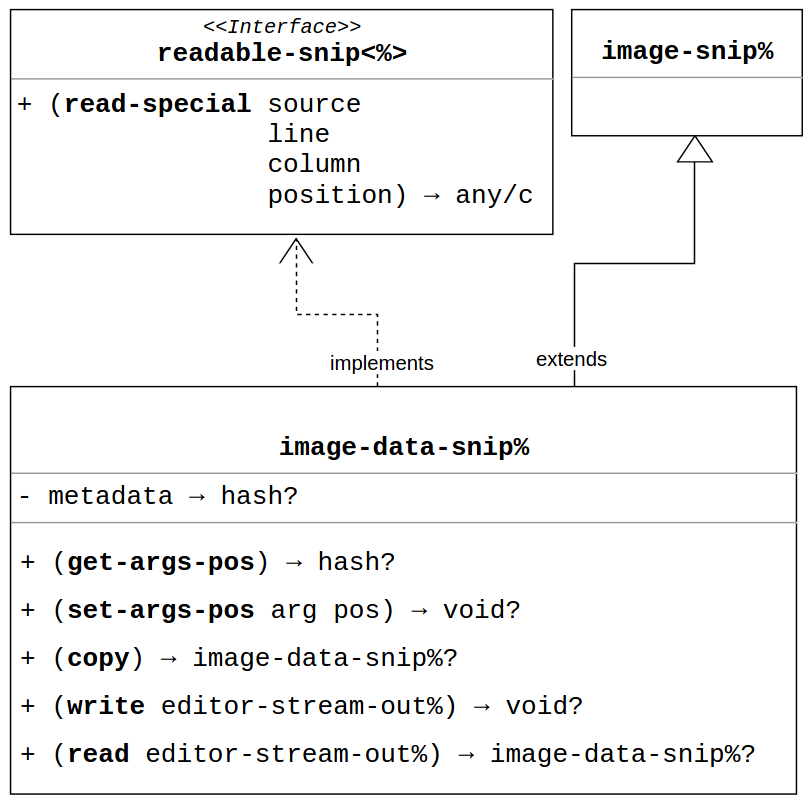
\includegraphics[scale=0.25]{images/img-data-snip}
    \caption{The UML diagram of the implemented class, \texttt{image-data-snip\%}. This class extends the original DrRacket snip class, and implements its own read syntax method.}
    \label{fig:img-data-snip}
\end{figure}

Because \texttt{image-data-snip\%} is a subclass of \texttt{image-snip\%}, it saves code and its associated metadata in ASCII-encoded binary format. This class uses the superclass method to store the image, but the methods for copying, reading, and storing the metadata field, were implemented from scratch. Unfortunately, the final serialized file does not provide backwards-compatibility among other text editors. However, the effort to implement this feature was more acceptable when considering the approach suggested in Chapter~\ref{chapter:pegd}.

Despite the beginning effort spent to implement this class, other features can benefit from this work. For example, the feature for expanding/collapsing images was applied on top of this class using only a few lines of code. Once the subclass already provides a method for resizing snips, this feature does a simple, super class call to change the size of the snip window. Moreover, this class defines a basis for other features that manipulates, or even edits, the image inserted in the text editor. 

\subsection{Auto Run}

The core of AutoRun \textit{plugin} is based on the snip of code shown in Listing~\ref{lst:callback}. This sample of code registers a pair of procedures with DrRacket’s online expansion machinery. The first two arguments name a method in a module that is loaded by dynamic-require. When DrRacket detects that the editor has been modified, it sends the contents of the editor to that separate place, expands the program there, and then supplies the fully expanded object. Then, this procedure (defined at line 4-7) gets the DrRacket editor frame (at line 6) and executes the code in that frame using the \texttt{execute-callback} function (at line 7). Therefore, upon a change in the text editor, DrRacket will execute the code immediately. 

\begin{lstlisting}[
language={[Auto]Lisp},
basicstyle=\ttm,
numbers=left,
stepnumber=1,
numbersep=5pt,                   
numberstyle=\scriptsize, 
caption={Executing the program through DrRacket execute-callback.},
label={lst:callback},
captionpos=b, 
otherkeywords={point,define,send},       % Add keywords here
keywordstyle=\ttb\color{black},
emph={define-syntax},       % Custom highlighting
emphstyle=\ttb\color{black},    % Custom highlighting style
stringstyle=\color{deepgreen},
numberstyle=\tiny\color{gray!110},
rulecolor=\color{gray!30},
frame=tb,                         % Any extra options here
showstringspaces=false,
backgroundcolor=\color{gray!5}            % 
]
(drracket:module-language-tools:add-online-expansion-handler
  online-comp.rkt
  'go
  (lambda ()
    (...) ;collapsed code
    (define drr-frame (send (send defs-text get-tab) get-frame))
    (send drr-frame execute-callback)))
\end{lstlisting}

When this \textit{plugin} is installed, it can become quite evasive once it is running code without the user permission. To avoid this situation, the \textit{plugin} is installed as a button in DrRacket's toolbar, having two operating modes. First, it is in disabled mode, which means that users can edit the code as before, and this \textit{plugin} will have no effect in DrRacket. Second, when it is on enable mode, it tries to execute the code at each change. However, to change the \textit{plugin} methods, users must authorize it, by clicking in the \textit{plugin} button.

Finally, to improve this tool an interactive mechanism to give inputs to the program was implemented, using the DrRacket slider widget. In this way, when a program literal is selected, and a keybinding is pressed, a slider appears on top of that literal. So, when the slider is dragged, the editor changes, which causes the AutoRun \textit{plugin} to execute the code. 

Unfortunately, adapting the range of values in the slider, interactively as users drag it, becomes difficult or even impossible to implement, using the DrRacket slider. To create a new slider is necessary to define the range and the initial value of that slider. However, to update these initial values, after the slider window is shown, the frame must be closed and opened again, which goes against the purpose of this tool.

\section{Conclusion}

Based on the ideas proposed in Chapter~\ref{chapter:pegd}, this chapter evaluates them, showing a coherent implementation. Then, it highlights the decisions made during the development of these tools, as well as the system used as a basis for implementation. Moreover, it shows the achieved results, presenting the architecture of the solution, the problems found, and how we overcame them. Next chapter shows a practical experiment conducted with these tools.